
\documentclass{article}
\usepackage[utf8]{inputenc}
\usepackage{geometry}
    \geometry{
    left=0.5in,
    top=0.5in,
    right=0.5in,
    bottom=0.75in
    }
\usepackage{enumitem} % https://latex.org/forum/viewtopic.php?t=28712
\usepackage{mdframed}
\usepackage{listings}
\usepackage{graphicx}
\graphicspath{ {../../common_images/} {./images/} {.} }
\usepackage{hyperref}
\hypersetup{colorlinks,urlcolor=blue}

\usepackage{soul} % strikethrough with \st{}

\usepackage{amsmath}  % for the recurrences with multiple cases

\usepackage{xcolor}

\definecolor{codegreen}{rgb}{0,0.6,0}
\definecolor{codegray}{rgb}{0.5,0.5,0.5}
\definecolor{codepurple}{rgb}{0.58,0,0.82}
\definecolor{backcolour}{rgb}{0.95,0.95,0.92}

\lstdefinestyle{mystyle}{
    backgroundcolor=\color{backcolour},   
    commentstyle=\color{codegreen},
    keywordstyle=\color{magenta},
    numberstyle=\tiny\color{codegray},
    stringstyle=\color{codepurple},
    basicstyle=\ttfamily\footnotesize,
    breakatwhitespace=false,         
    breaklines=true,                 
    captionpos=b,                    
    keepspaces=true,                 
    numbers=left,                    
    numbersep=5pt,                  
    showspaces=false,                
    showstringspaces=false,
    showtabs=false,                  
    tabsize=2
}

% \lstdefinestyle{mystyle}{
%     basicstyle=\ttfamily\footnotesize,
%     breakatwhitespace=false,         
%     breaklines=true,                 
%     captionpos=b,                    
%     keepspaces=true,                 
%     numbers=left,                    
%     numbersep=5pt,                  
%     showspaces=false,                
%     showstringspaces=false
% }
 
\lstset{style=mystyle}

% Source: https://tex.stackexchange.com/questions/30720/footnote-without-a-marker
\newcommand\blfootnote[1]{%
  \begingroup
  \renewcommand\thefootnote{}\footnote{#1}%
  \addtocounter{footnote}{-1}%
  \endgroup
}

% https://www.overleaf.com/learn/latex/Questions/How_do_I_tab_(indent)_a_paragraph_in_LaTeX%3F
\usepackage{indentfirst}

\title{ECS 32B: Conceptual Homework \#3}
\author{Instructor: Aaron Kaloti}
\date{Summer Session \#2 2020\blfootnote{This content is protected and may not be shared, uploaded, or distributed.}}

\begin{document}

\maketitle

% \tableofcontents

\section{Changelog}

You should always refer to the latest version of this document.

\begin{itemize}[itemsep=0mm, parsep=0pt]
\item v.1: Initial version.
\item v.2: For the first problem, you should specify the height and balance factor of each node in the final tree of each subproblem.
\item v.3: Clarified about duplicates (no duplicate keys allowed) for problem \#3.
\item v.4: Fixed initial tree in problem \#1. (Or, rather, unbroke it, since I think it was fine at least in the initial version but somehow got messed up along the way.)
\end{itemize}

\section{Grading}

\begin{itemize}[itemsep=0mm, parsep=0pt]
\item \textbf{Due date: 5:00 PM on Wednesday, 09/09. There is no ``grace period.''}
\item A subset of the problems will be graded for correctness. The rest will be graded on completion.
\end{itemize}

\section{Submission Requirements}

\begin{itemize}[itemsep=0mm, parsep=0pt]
\item Your submission must be typed with LaTeX. \textbf{Handwritten/scanned solutions, or solutions not typed with LaTeX, will earn no credit.}
    \begin{itemize}[itemsep=0mm, parsep=0pt]
    \item You should avoid doing this assignment at the last minute, because it will take a bit of time to get used to LaTeX and to type your answers up into a LaTeX document.
    \end{itemize}
\item Your submission must consist of one file, the PDF generated by your LaTeX file (\lstinline{hw3_answers.pdf}). Since Gradescope does not let you submit files that are neither PDFs nor images, I will not have you submit the \lstinline{.tex} file. However, if it is clear that your submission was not made with LaTeX, we may email you to ask that you send us your \lstinline{.tex} file, and if you cannot (i.e. if it turns out that your PDF was in fact not created with LaTeX), you will get a zero on this assignment.
\item You may be penalized if, when submitting on Gradescope, you mark the wrong page for a given homework problem, because dealing with this slows down grading. In the middle of the 08/06 lecture, I talk about how to mark the pages of your submission on Gradescope, starting at around 1:03:55 in the video.
\item When using LaTeX, you should make use of the math notation/mode where sensible. (The math mode refers to when you put mathematical equations, etc. between dollar signs so that LaTex makes them look nice.) Repeated failures to do this, to the point that the purpose of using LaTeX is defeated or the readability of your answers is impeded, may result in a penalty on this assignment.
\end{itemize}

\section{Regarding Collaboration}

\begin{itemize}[itemsep=0mm, parsep=0pt]
\item You may not copy answers from any sources, including online sources such as Chegg, StackOverflow, or any solutions manual of any textbook.
\item You may partner with \textbf{\textit{at most one}} other student on this assignment. In other words, you can work in \textit{pairs}. You do not have to partner with anyone. (In fact, I think it is better that you do not.) If you partner with someone, it must be a committed partnership; that is, you two will have the same submission, and you must mark on Gradescope that you have partnered for this assignment by following the directions \href{https://www.youtube.com/watch?v=rue7p_kATLA}{here}.
\item If students that were not in the same pair seem to have excessively similar answers, they will be reported to the OSSJA for suspicion of academic misconduct. Do not copy answers from (or share answers with) any student who you are not partnered with.
\end{itemize}

\section{Identification}

Enter the members of your pair. (You can partner with at most one other student.) If you are not partnered with anyone, then leave the second box empty. You can remove the use of \lstinline{\vspace} in the \lstinline{.tex} file.

Pair member \#1:

\begin{mdframed}
\vspace{3em}
%% TODO
\end{mdframed}

Pair member \#2:

\begin{mdframed}
\vspace{3em}
%% TODO
\end{mdframed}

\section{Problems}

For the problems in which you have to draw something, you can insert an image of your drawing with \lstinline{includegraphics}; see more details in the ``AVL Tree Insertion'' problem section.

Whenever I say that you must draw a tree, you don't have to handwrite it, i.e. you could use some software for drawing if you want. However, you must actually draw a tree; don't alternatively provide some list of the nodes and edges, or you won't get credit.

\subsection{AVL Tree Insertion}

\subsubsection{Insert $40$}

Show the AVL tree that results from inserting $40$ into the below AVL tree. If you wish, you can draw the tree by hand and, after uploading an image of, include said image with \lstinline{includegraphics}; see how it's used in the LaTeX file to include the image of the original tree, and note that the file extension must be omitted.) \textcolor{red}{You must specify the height and balance factor of each node in the final tree.}

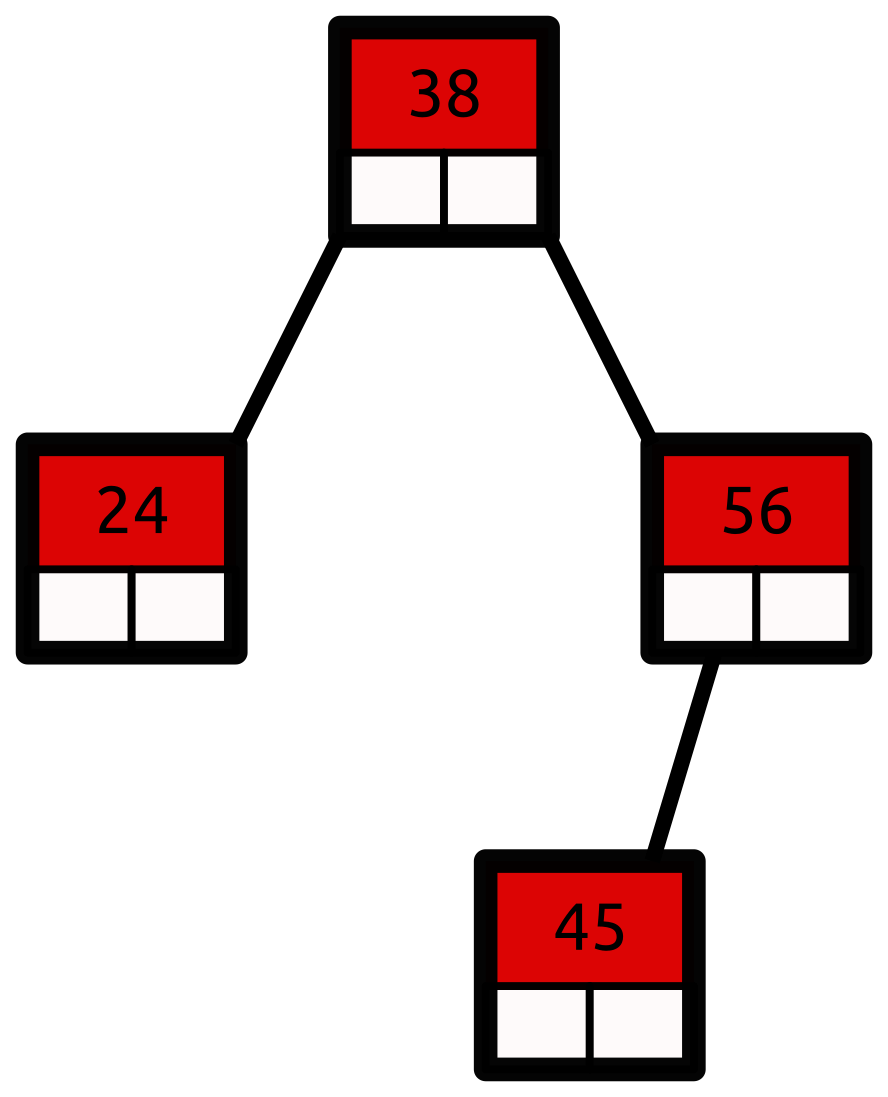
\includegraphics[scale=0.35]{avl_tree_insert_problem}

\begin{mdframed}
\vspace{3em}
%% TODO
\end{mdframed}

\subsubsection{Insert $64$}

Show the AVL tree that results from inserting $64$ \textit{into the AVL tree that you have as your answer above}. \textcolor{red}{You must specify the height and balance factor of each node in the final tree.}

\begin{mdframed}
\vspace{3em}
%% TODO
\end{mdframed}

\subsection{AVL Trees: Professor Mean Dude}

Professor Mean Dude is currently teaching a Python data structures course this summer and is trying to create a very hard final exam. One of the questions that he is working on is meant to test students' knowledge of AVL tree insertion and rebalancing. This question (the one that he created) asks what should happen if the key $80$ is inserted into the tree shown below.

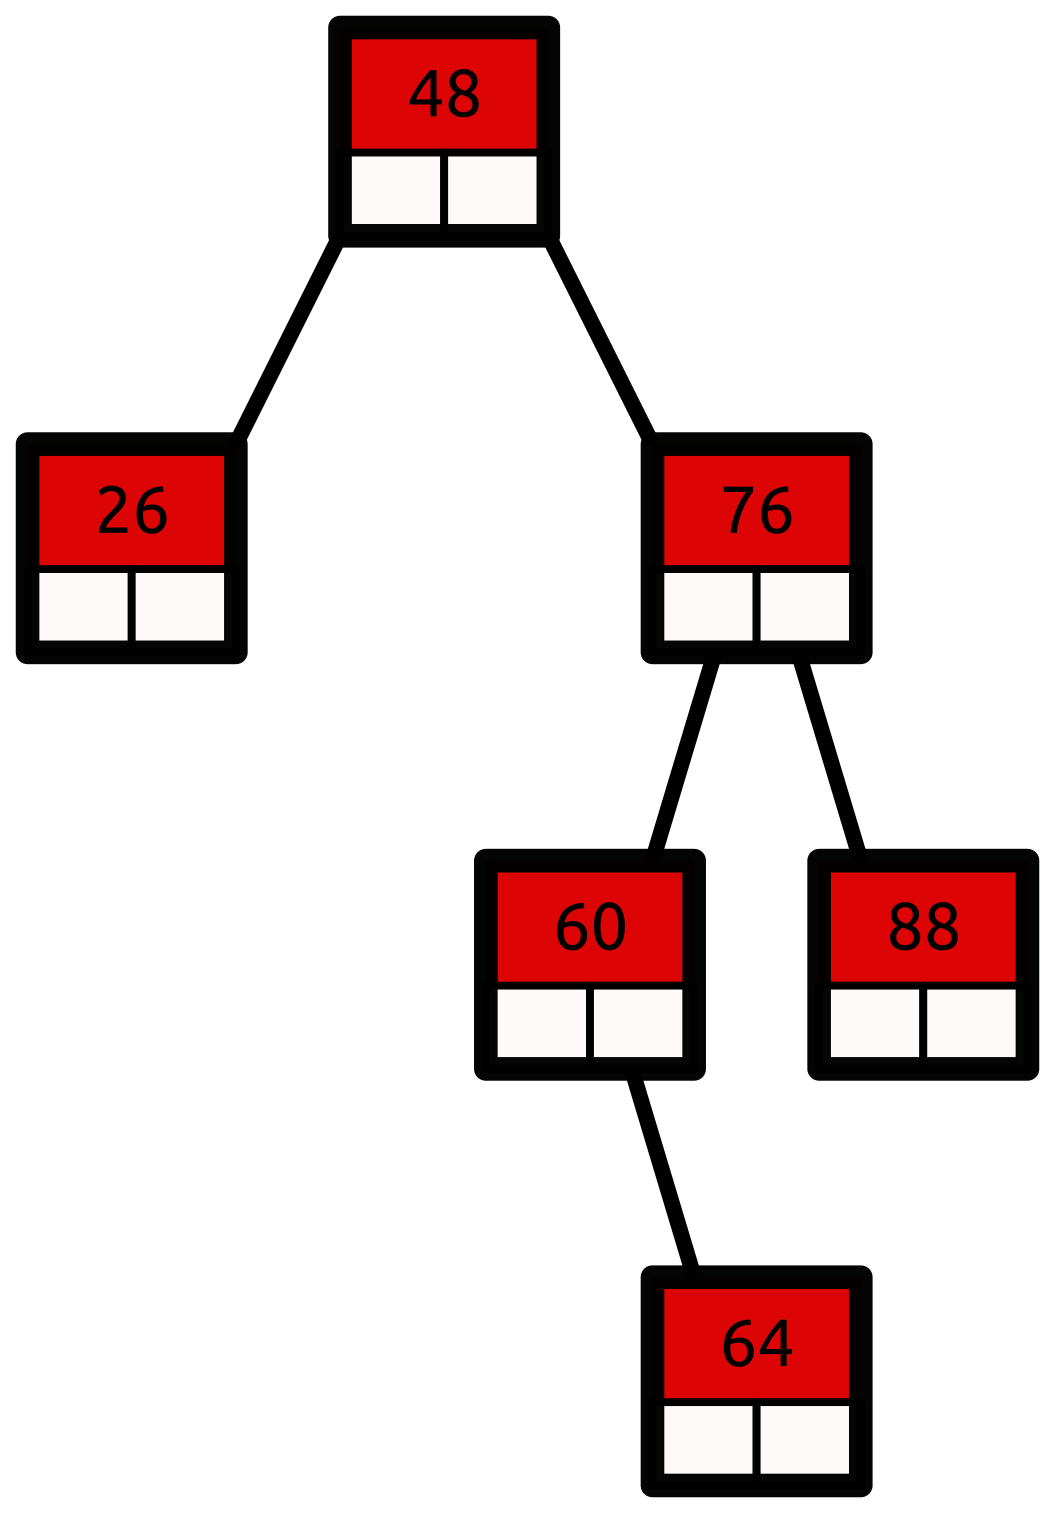
\includegraphics[scale=0.3]{prof_mean_dude_avl_tree}

Unfortunately, after inserting $80$, Professor Mean Dude is not sure how to rebalance the tree. Following the rules on slide \#9 of slide deck \#7, the balance factor of $80$ is $0$, the balance factor of $88$ becomes $1$, and the balance factor of $76$ becomes $0$. Since a node whose balance factor became $0$ is encountered, no more updating should occur, as stated on slide \#10. However, Professor Mean Dude notices that the tree is still unbalanced, even though he followed the rules on the lecture slides. What did Professor Mean Dude do wrong? Did Professor Mean Dude perform the insertion wrong? Or is there another issue? Explain.

\begin{mdframed}
\vspace{3em}
%% TODO
\end{mdframed}

\subsection{AVL Trees: Range of Bad Insertions}

Consider the AVL tree below. Suppose that we are inserting an \textit{integer} $x$ into the tree. What is the range of values that $x$ can take on such that inserting $x$ will result in a rebalancing (i.e. either a single rotation or double rotation) somewhere in the tree? You may assume that $0 \le x \le 100$, and you may assume that \textbf{no duplicate keys are allowed}.

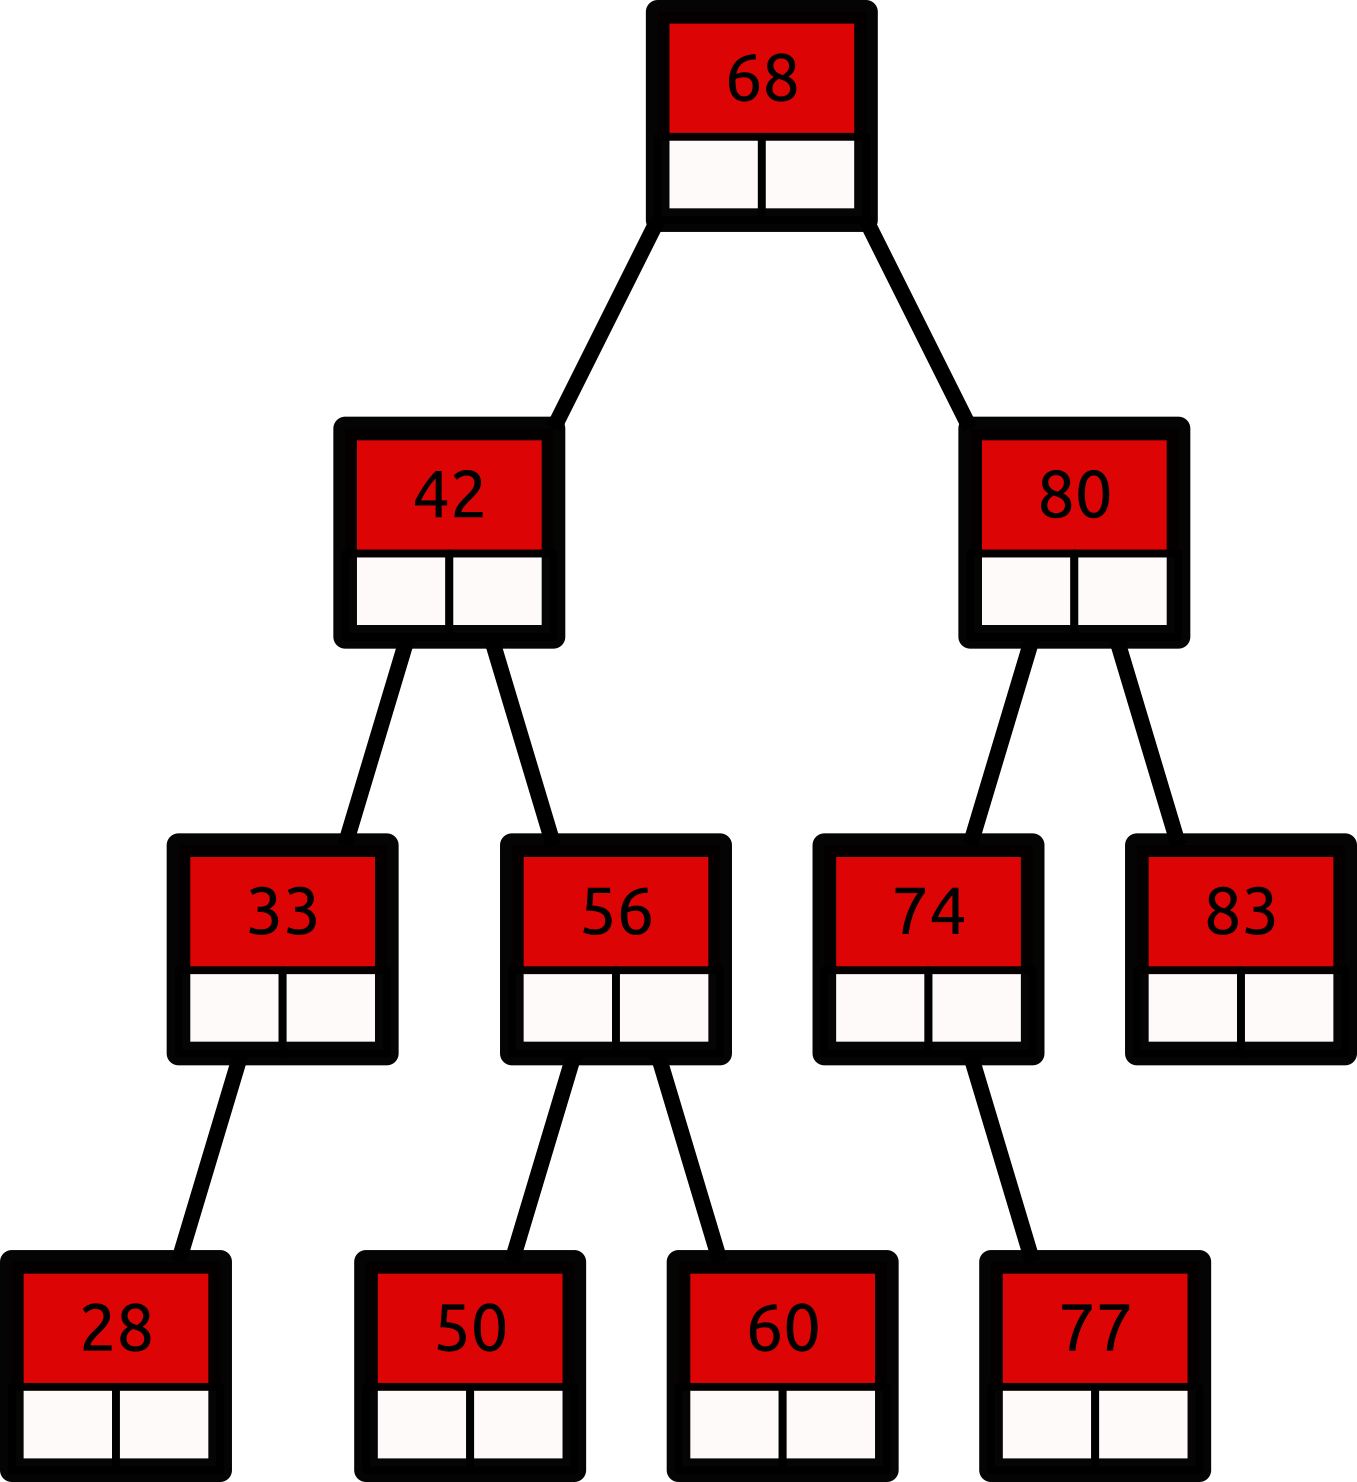
\includegraphics[scale=0.35]{avl_tree_range_problem}

\begin{mdframed}
\vspace{3em}
%% TODO
\end{mdframed}

Below is a tip on how to express the range. If you are trying to express that $x$ is either in between $38$ and $52$ (inclusive) or in between $67$ and $78$ (with $78$ excluded), then you can express this range like so (see how it's done in the \lstinline{.tex} file):

$[38,52]\cap[67,78)$

\subsection{AVL Trees: Two Deletions}

In this problem, you will create an AVL tree of integers and specify an integer $x$ to delete from your tree, subject to the following conditions:

\begin{itemize}[itemsep=0mm, parsep=0pt]
\item $x$ is a leaf in the AVL tree.
\item Deleting $x$ results in two rebalances (in the order given):
    \begin{itemize}[itemsep=0mm, parsep=0pt]
    \item A left single rotation.
    \item A right-left double rotation.
    \end{itemize}
\item Your AVL tree has as few nodes as is necessary to fulfill the above conditions.
\end{itemize}

You must provide the following:

\begin{itemize}[itemsep=0mm, parsep=0pt]
\item The original AVL tree.
\item The integer to delete.
\item The AVL tree after performing the first rebalance, i.e. the left single rotation.
\item The AVL tree after performing the second rebalance, i.e. the right-left double rotation.
\end{itemize}

\begin{mdframed}
\vspace{3em}
%% TODO
\end{mdframed}

\subsection{Splay Tree Insert and Find}

Consider the splay tree shown below.

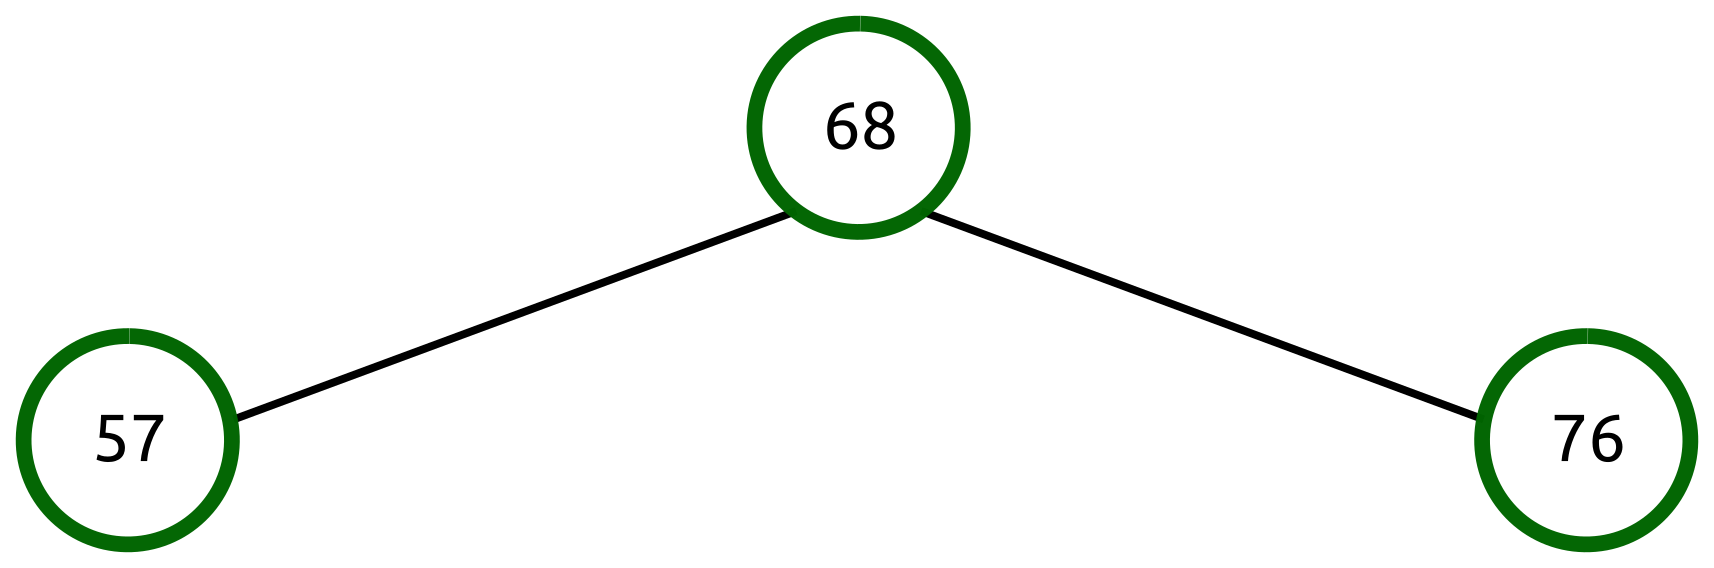
\includegraphics[scale=0.3]{splay_tree_insert_problem}

For each problem below, a splay tree operation is given. Draw the splay tree that results from doing that operation on the splay tree. The operations are cumulative, e.g. the third operation is performed on the tree that you got from the second operation. As with the earlier AVL tree problem, you may want to use \lstinline{includgraphics} to insert an images of your drawings.

\subsubsection{Insert $40$}

\begin{mdframed}
\vspace{3em}
%% TODO
\end{mdframed}

\subsubsection{Insert $70$}

\begin{mdframed}
\vspace{3em}
%% TODO
\end{mdframed}

\subsubsection{Find $68$}

\begin{mdframed}
\vspace{3em}
%% TODO
\end{mdframed}

\subsubsection{Insert $45$}

\begin{mdframed}
\vspace{3em}
%% TODO
\end{mdframed}

\subsection{$d$-Heaps}

A $d$-heap is a generalization of a binary heap that is exactly the same as a binary heap, except that each node has $d$ children. Thus, a binary heap is a $2$-heap, and a ternary heap is a $3$-heap.

\subsubsection{One-Based Indexing}

Recall that a binary heap can be represented as a Python list. Given a node at index $i$ in this Python list, the formulas for finding the index of the parent and left/right children of this node (assuming one-based indexing) were given during lecture. Suppose we are implementing a Python list representation of a ternary heap. Given a node at index $i$ in this Python list, give the formula for finding the index of the parent, and give the formulas for finding each of the children of this node.

\begin{mdframed}
\vspace{3em}
%% TODO
\end{mdframed}

\subsubsection{Zero-Based Indexing}

Repeat the previous problem, except with zero-based indexing instead (i.e. the root of the ternary heap is at index 0 in the Python list).

\begin{mdframed}
\vspace{3em}
%% TODO
\end{mdframed}

\subsection{Caching}

Computer architecture, and more specifically computer memory, is a complex and interesting subject in which, as in software-oriented areas like data structures and algorithms, there are many common problems to solve and many tradeoffs to make for speed and other considerations. One such tradeoff is between speed and cost (of making the hardware) and involves what is called the \textit{memory hierarchy}. An abbreviated image of the memory hierarchy is shown below.

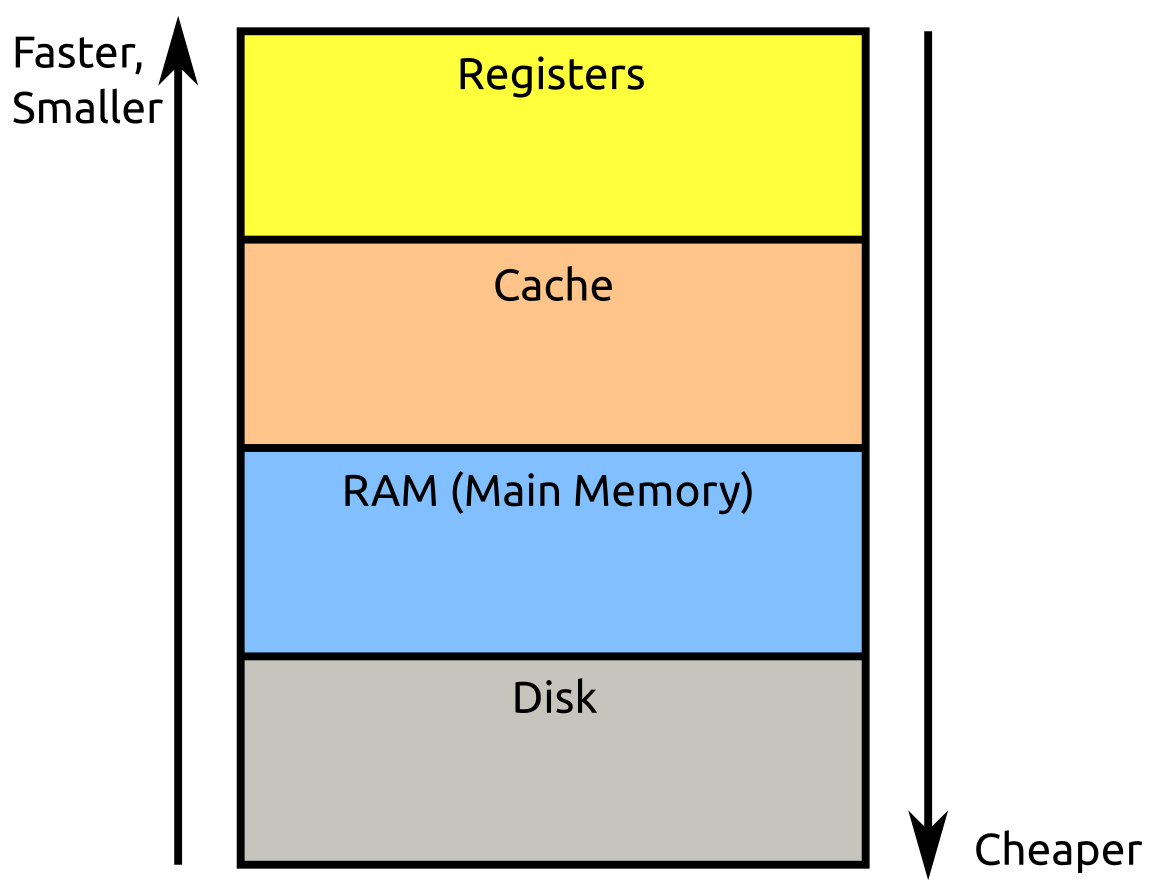
\includegraphics[scale=0.4]{memory_hierarchy}

Certain properties can make one kind of memory faster (and more expensive) than another kind of memory. Consequently, the registers and cache are the fastest kinds of memory in your computer, whereas the disk is the most plentiful. When a program needs to access a certain piece of data from memory, it will first try to access that data from the cache (prounounced ``cash'')\footnote{I don't think explaining registers will make much sense until you've used a compiled programming language such as C or C++}. If that fails, then main memory will be checked next, and if that fails, then the disk will be checked. It would be ideal if any data needed by our program happened to be in the cache, but since the cache has a limited size (and since our Python program is not the only software running on our computer), this is impractical. Thus, a cache must be careful about which data is stored. One common rule is to store, in the cache, any data (from main memory or disk) that was recently accessed. The idea behind this is the same as the motivation behind a splay tree: data that was recently accessed is more likely to be accessed again. Cache designers took this idea even further by observing the principle of \textit{spatial locality}: when a program such as a Python program accesses index $i$ in an array $A$ (or a ``list'' or ``Python list'', as we call it in Python), where the elements are contiguous, it is likely that indices $i + 1$, $i + 2$, $i + 3$, and some more beyond that are likely to be accessed soon (think of a \lstinline{for} loop iterating through a list like \lstinline{[5,8,14,2,9]}; the chance that you access \lstinline{8} after having accessed \lstinline{5} is quite high). Thus, in this scenario, a cache that takes advantage of spatial locality would store not only the recently accessed $A[i]$ in the cache but also store $A[i + 1]$, $A[i + 2]$, $A[i + 3]$, and perhaps several more elements along with it\footnote{The exact number depends on factors we will not get into, but certainly, the cache cannot grab all the elements that it wants to; there are limits.}, since those elements are right after $A[i]$ anyways and do not take significant additional time to grab. Importantly, spatial locality can be taken advantage of here \textit{because $A[i], A[i+1], A[i+2], A[i+3], ...$ are contiguous in memory}; if they were not, then spatial locality would be irrelevant.

\subsubsection{Python List vs. Linked List}

Which of a normal list (i.e. a Python list) vs. a linked list would you expect to benefit more from a cache taking advantage of spatial locality? Explain.

\begin{mdframed}
\vspace{3em}
%% TODO
\end{mdframed}

\subsubsection{Separate Chaining vs. Open Addressing}

With a hash table, with which of separate chaining (with a linked list) vs. open addressing (with linear probing) would you expect to benefit more from a cache taking advantage of spatial locality? Explain.

\begin{mdframed}
\vspace{3em}
%% TODO
\end{mdframed}

\subsubsection{Linear Probing vs. Quadratic Probing}

With a hash table using open addressing, with which of linear probing vs. quadratic probing would you expect to benefit more from a cache taking advantage of spatial locality? Explain.

\begin{mdframed}
\vspace{3em}
%% TODO
\end{mdframed}

\subsection{Check Duplicates}

Suppose that you are writing a function that checks if a list of values contains any duplicate values. That is, the function should return \lstinline{True} if the list does and \lstinline{False} otherwise. \textbf{What would be the worst-case time complexity of each of the approaches to this function? Explain. Where it would help your explanation, you might want to explain what a worst-case scenario would be for that specific approach and/or use one of the two summations mentioned below.} In some cases, I use classes that you may assume do what the names suggest, e.g. \lstinline{HashTable}, and fake method names that also do what their names suggest, e.g. \lstinline{insert()}; this is not valid Python, since those classes are not built-in. You should make sure to not assume the \lstinline{in} operator always has the same worst-case time complexity (e.g. linear time, constant time) no matter what the data structure is. Although the hash table operations \lstinline{find}, \lstinline{insert}, and \lstinline{delete} take \textit{amortized} constant time, you will not be penalized for omitting the word ``amortized'' in your analysis.

You may find these summations helpful. The first one was described during the lecture on selection sort and insertion sort. You can take these as fact, i.e. you don't have to prove them. \textit{You may find it appropriate to mention these summations in your analysis when appropriate.} Consequently, you should understand \textit{why} the first summation was used in the worst-case analysis of selection sort.

\begin{itemize}
\item $\sum\limits_{i=1}^{n} i = \Theta(n^2)$.
\item $\sum\limits_{i=1}^{n} \lg i = \Theta(n \lg n)$.
\end{itemize}

\subsubsection{Nested Loops}

\begin{lstlisting}[language=Python]
def HasDuplicate(vals):
    for i in range(len(vals)):
        for j in range(i + 1, len(vals)):
            if vals[i] == vals[j]:
                return True
    return False
\end{lstlisting}

\begin{mdframed}
\vspace{3em}
%% TODO
\end{mdframed}

\subsubsection{Binary Search Tree}

\begin{lstlisting}[language=Python]
def HasDuplicate(vals):
    bst = BST()  # create instance of binary search tree
    for val in vals:
        if val in bst:
            return True
        bst.insert(val)
    return False
\end{lstlisting}

\begin{mdframed}
\vspace{3em}
%% TODO
\end{mdframed}

\subsubsection{AVL Tree}

Same as the previous part, except that \lstinline{bst} is an instance of \lstinline{AVLTree} instead of of \lstinline{BST}.

\begin{mdframed}
\vspace{3em}
%% TODO
\end{mdframed}

\subsubsection{Hash Table}

\begin{lstlisting}[language=Python]
def HasDuplicate(vals):
    h = HashTable()
    for val in vals:
        if val in h:
            return True
        h.insert(val)
    return False
\end{lstlisting}

Specify the worst-case time complexity in terms of the length of the input list only, not the size of the hash table.

\begin{mdframed}
\vspace{3em}
%% TODO
\end{mdframed}

\subsection{Sorting Algorithms: Best-Case Analysis}

For each of the following sorting algorithms, is there a meaningful distinction between the ``best case'' and the ``worst case''. That is, would the best-case time complexity differ from the worst-case time complexity? If it does differ from the worst-case time complexity, then explain why and, if it helps your explanation, give an example of an input that would cause the best case to occur. If the best-case time complexity \textit{does not} differ, then just say that it does not differ (e.g. ``No difference.'') without any elaboration.

\subsubsection{Bubble Sort}

\begin{mdframed}
\vspace{3em}
%% TODO
\end{mdframed}

\subsubsection{Selection Sort}

\begin{mdframed}
\vspace{3em}
%% TODO
\end{mdframed}

\subsubsection{Insertion Sort}

\begin{mdframed}
\vspace{3em}
%% TODO
\end{mdframed}

\subsubsection{Mergesort}

\begin{mdframed}
\vspace{3em}
%% TODO
\end{mdframed}

\begin{center}

\includegraphics[scale=0.4]{UCD_CS_Logo}
\end{center}

\end{document}
